\documentclass[tikz,border=10pt]{standalone}
% No TikZ libraries needed for this figure.
\begin{document}
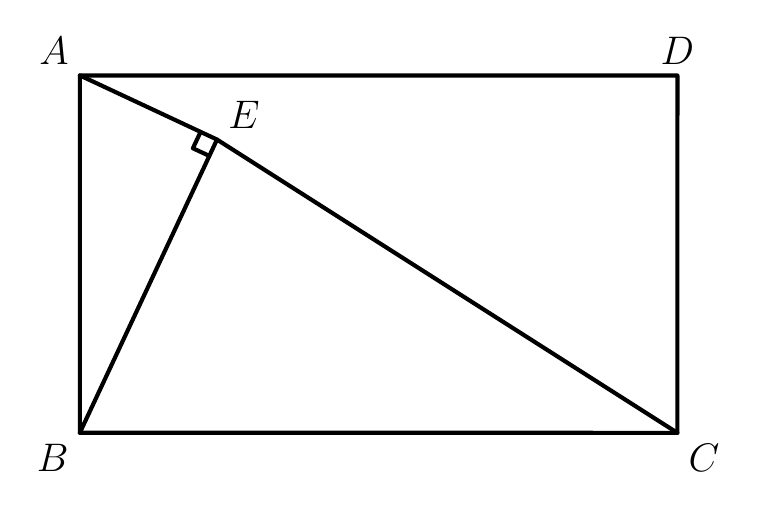
\begin{tikzpicture}[line width=1.5pt, line join=round, line cap=round]
  % Named coordinates: scale s = 0.019324 cm/px, origin at rectangle centre (244,182.5) px
  \coordinate (A) at (-3.7911006068305886,2.2717178728764837);
  \coordinate (B) at (-3.7918365789599937,-2.26612545560783);
  \coordinate (C) at (3.796632267825599,-2.2673561947876144);
  \coordinate (D) at (3.797368239955005,2.2704871336966987);
  \coordinate (E) at (-2.05006332199002,1.4572766438222615);

  % Rectangle ABCD (solid)
  \draw (A) -- (B) -- (C) -- (D) -- cycle;

  % Segments AE and EC (bend at E), and BE
  \draw (A) -- (E) -- (C);
  \draw (B) -- (E);

  % Right-angle marker at E (one mark, on the EA/EB wedge)
  \draw (-2.2585274852983575,1.5544323300265919) -- (-2.3560371351218365,1.3466717557636725) -- (-2.1475729718134993,1.249516069559342);

  % Labels
  \node[above left]  at (A) {\fontsize{15.5}{18.6}\selectfont $A$};
  \node[above]       at (D) {\fontsize{15.5}{18.6}\selectfont $D$};
  \node[below left]  at (B) {\fontsize{15.5}{18.6}\selectfont $B$};
  \node[below right] at (C) {\fontsize{15.5}{18.6}\selectfont $C$};
  \node[above right] at (E) {\fontsize{15.5}{18.6}\selectfont $E$};
\end{tikzpicture}
\end{document}